\documentclass[man,noapacite]{apa2} 

\usepackage{apacite2}
\usepackage{amssymb}
\usepackage{graphicx}

\title{Using Tablets to Collect Data from Young Children} 

\fiveauthors{Michael C. Frank}{Elise Sugarman}{Alexandra Horowitz}{Molly L. Lewis}{Daniel Yurovsky} 

\fiveaffiliations{Department of Psychology, Stanford University}{Department of Psychology, Stanford University}{Department of Psychology, Stanford University}{Department of Psychology, Stanford University}{Department of Psychology, Stanford University}

\abstract{Mobile, touch-screen devices are increasingly ubiquitous in children's lives. The extensive use of such devices provides both a challenge and an opportunity for developmental psychologists. While more research is needed to understand the nature and consequences of young children's interaction with such devices, they nevertheless present an exciting opportunity for data collection. We present a simple method for creating cross-platform, interactive tablet experiments using open web-based resources. We illustrate this method by collecting data from children 1--5 years old in a simple word-recognition paradigm and show that this method yields reliable reaction time and accuracy data from very young children. Tablets should be considered by researchers as a viable method for collecting low-cost, well-controlled developmental data.}

\shorttitle{Tablet-based Data Collection} 
\rightheader{TABLET-BASED DATA COLLECTION}

\acknowledgements{We gratefully acknowledge the laboratory of Anne Fernald for sharing their stimuli and the families and staff at San Jose Children's Discovery Museum. An earlier version of this material was previously presented in a blogpost \cite{blog}. Thanks to Janelle Klaas, Andrew Weaver, and Sarah James for assistance in data collection. Please address all correspondence to Michael C. Frank, Department of Psychology, Jordan Hall (Bldg. 420), 450 Serra Mall, Stanford, CA 94305. Phone: (650) 724-4003. E-mail: \texttt{mcfrank@stanford.edu}}

\begin{document}

\maketitle

%\setlength{\textfloatsep}{0.02cm}

\section{Introduction}

Since Apple debuted the iPad in 2010, the ubiquity of personal tablets---interactive, touchscreen-based computing devices, typically larger than a phone but smaller than a laptop---has skyrocketed. By 2013, an estimated 75\% of families with young children in the United States owned a mobile device, with 40\% of households owning tablets (20\% of lower-income families and 63\% of higher-income families) \cite{rideout2013}. At present, tablets are estimated to constitute 19\% of children’s overall screen time from ages 0--8. This explosion in popularity has created a surge of interest in both the consequences of tablet use for children and the potential for using these devices as scientific tools. 

Nevertheless, there are significant challenges involved in using tablets for research. These include the difficulty and potential costliness of developing custom applications (``apps'') for individual experiments, technical problems with app distribution and cross-device compatibility, and the lack of data confirming the validity of the tablet data collection method. Perhaps for these reasons, at the time of writing there is a paucity of published articles that use tablets to collect developmental data. 

The goal of the current article is to address these challenges. We begin by briefly reviewing research on the use of tablets in children. We then describe a method for using standard, freely-available web-development tools to create tablet-based experiments. Although this method requires some programming experience, it is significantly easier than developing tablet-native applications and has relatively few drawbacks from the research perspective. We next show how this method can be used to implement a simple word-recognition experiment. Our data suggest that the tablet platform is an engaging method for data collection that yields reliable accuracy and reaction time from children two years old and perhaps even younger. 

\section{Children's Tablet Use}

Children's ability to learn from entertainment technologies is contested. A number of influential studies suggest that children learn less from videos than they do from live demonstrations, a phenomenon known as the video deficit effect (e.g. Anderson \& Pempek, 2005; DeLoache et al., 2010; Kuhl et al., 2003). Additionally, Zimmerman et al. (2007) surveyed parents reports of television-viewing and childrens vocabulary under age 2 and found that infants who spent more time viewing infant-directed programs (“baby media, such as the Baby Einstein series), the lower their reported vocabulary (although see Ferguson \& Donnellan (2014) for a recent reevaluation and extension of this work suggesting a null relationship between educational programming and vocabulary development). These findings suggesting negative relationships between screen viewing and vocabulary growth influenced the American Academy of Pediatrics (AAP) to uphold a policy recommending no screen time for children under age 2 (Brown, 2011).

Although screen media tends not to offer as rich pedagogical experiences as live interactions, touch-screen mobile devices may stand apart from traditional view-only screens. Unlike video programming, touch-screens offer an interactive experience with contingent feedback to childrens touch input, and a range features that can be individualized to a childs age and performance. In fact, Christakis (2014) notes that the AAPs published media recommendation of no screen time was made before the release of tablet devices, and suggests that the policy should be revised to distinguish and accommodate some time with touch-screens. He proposes that tablets can offer a number of potential benefits that, individually, many traditional toys do not. Specifically, tablets are reactive (responding contingently to the child’s actions), interactive (eliciting responses from the child based on his or her actions), tailorable (modified according to age or other preference), progressive (can increase in difficulty or complexity with experience), highly portable, and able to promote joint attention (a child and caregiver can interact with the program together). While no screens are not recommended as replacements for live interactions, interactive technologies may pose a number of benefits over other passively-viewed screen alternatives. Some work suggests that practice with interactive games may benefit attention and motor control (Bavelier et al., 2010), and more generally screen time with tablets can promote independence, opportunities for physical closeness, and feelings of fun and accomplishment (Rvachew, 2014). The contingent feedback and individualization offered by mobile devices may make them better mediums for learning and engagement than traditional view-only screens, and also valuable tools for research and evaluation.

Young children do demonstrate some learning from interactive screen content, suggesting that the video deficit effect may be limited to---or at least strongest in---passive viewing of pre-recorded material. In one study, \citeA{roseberry2014} found that 24- to 30-month-olds successfully learned a novel verb from a live interaction via video chat, while a yoked group who saw the same input with non-contingent presentation failed to learn.
% They taught 24- to 30-month-olds novel verbs in one of three conditions: in-person demonstration, video chat demonstration, or a yoked video demonstration (recorded from a different child, therefore not socially-contingent to the participant). They found that toddlers were able to learn the new verbs above chance and equally well for both of the socially-contingent conditions (in-person and video chat demonstrations), but were only at chance in the control condition. Even despite challenges from in-person information (e.g. skewed gaze cues due to the position of the camera), the contingent feedback appears to drive children’s ability to learn through live video interactions.
Young children also show some evidence of transferring learning between screens and physical objects. \citeA{zack2009} examined 15-month-olds' ability to transfer knowledge learned via a touch-screen or physical toy to another example either in the same presentation modality or across modalities. They found that children were most successful when toys were presented in the same modality, but that children in the cross-modality conditions performed significantly better than a no-demonstration baseline. These findings suggest that even before age 2, children show evidence of comprehending actions and goals presented on touch-screen devices and can transfer this knowledge between physical and 2-dimensional presentations.


Although children show interest and remarkable capabilities to use touch-screens even before they learn to talk, some affordances of mobile tablets are easier to master from young ages than others. Aziz et al. (2014) tested 2- to 5-year-olds in Malaysia and the United Kingdom on their ability to perform the seven most common touch gestures of iPads: tap, drag/slide, free rotate, drag and drop, pinch, spread, and flick. By age 2, children mastered the tap and drag/slide gestures, and by age 3, they could reliably produce all by the spread gesture. By age 4, all children performed all of the gestures. One concern with childrens performance is the accuracy of their motor control. Couse \& Chen (2010) found that young children can quickly learn to provide precise motor input on tablets with minimal training using a stylus pen that can digitally write on the screen. They had teachers rate the quality and complexity of 3- to 6-year-olds self-portraits created digitally on a tablet art program compared with their drawing using traditional writing tools on paper. They found that children were highly engaged with tablet program, their drawings were rated as typical or exceeding their typical quality of drawing, and three quarters of children on the tablet task exhibited no to little frustration during the task despite a number of technical challenges. Additionally, researchers were prepared to give children up to four warm-up sessions using a stylus pen on tablet computer, but most children advanced after a single warm-up phase. Altogether, these studies suggest that children are highly motivated and competent at interacting with touch-screen tablets. Designers of iPad materials for young children should consider appropriate content and gesture capabilities according to the target age, and precision of touch input may be increased with tools such as fine-tipped stylus pens instead of finger touches.

\section{Collecting Developmental Data With Tablets}

\subsection{The Value of Tablet-Based Data Collection}

We offer five reasons why tablets may be valuable tools for developmental research.

\subsubsection{Diverse measures} Tablets allow the collection of many different dependent variables, including forced-choice responding, reaction time, and gesture trajectories.

\subsubsection{Engagement} Children across ages enjoy tablets and are highly motivated to explore new tablet-based tasks, allowing researchers to collect more data from individual children.

\subsubsection{Experimental control} Studies that involve interaction with an experimenter are the de-facto standard in cognitive development research, but such studies have as major drawbacks that it may be difficult or impossible to ensure that experimenters are blind to condition and hypothesis. While there are methods for avoiding such issues, the possibility of eliminating experimenter bias via computerized stimulus presentation is an attractive method for situations where it is possible. In addition, even when bias is not introduced, there are significant challenges in training a group of research assistants to implement an experimental protocol uniformly. 

\subsubsection{Inclusion of special populations} Tablets can be a valuable tool for working with children who have learning or physical disabilities, including ASD and dystopia (e.g. Cardon, 2012; Waddington et al., 2014; Chai et al., 2014; Bertucco \& Sanger, 2013)); 

\subsubsection{Scale} The low cost and high accessibility make it possible to distribute tablets to research assistants who can collect data in a wider variety of locations (though not without concern about environmental distractions). In addition, it is in principle possible that children could contribute data to experimental studies via experiments administered by their parents or caregivers.\footnote{For an example of this method, see \texttt{http://lookit.mit.edu}, a web-based platform for looking-time experiments that engages parents as experimental confederates.} It is this latter possibility that might be truly revolutionary in terms of the scope of data collection, though there are many challenges that such research would need to overcome.

% online application platforms may allow reachers to reach more diverse populations and collect data more rapidly). 

\subsection{Current methods for developing tablet experiments}

reating iPad apps requires mastering a framework and programming language that are specific to iOS, and putting the apps on more than a few iPads requires dealing with the app store. Neither of these are impossible hurdles, but both of them have kept us (and AFAIK most other labs) from getting very far in using them for routine day-to-day data collection.


\subsection{A web-based method for developing tablet experiments}

In contrast to these other methods, our recipe for experiment development is easy to use; makes use of free, industry-standard web development tools; does not require interaction with commercial app platforms; and  offers the ability to collect control data with adult participants on Amazon Mechanical Turk \cite{paolacci2010,crump2013} with virtually no changes. Our method has three components:

\begin{enumerate}
\item A JavaScript/CSS/HTML web experiment, 
\item A server-side PHP script to collect data in tabular format, and
\item A tablet device running a kiosk application. 
\end{enumerate}

\noindent We discuss each below.\footnote{Our work has used the Apple iPad as the primary tablet platform and we provide details that are tailored for this platform. Nevertheless, and unlike other methods, our method is in principle portable to a wide range of mobile devices with only very minor modifications.}

\subsubsection{Web-based experiment}

It is beyond the scope of this article to provide an introduction to creating JavaScript-based web experiments, but there are a wealth of available resources on this topic. These resources include both psychology-specific tutorials and more general introductions to the document-object model that has recently become the standard framework for constructing websites. A sample experiment (as well as the server side code) is provided in the version control repository for this paper (\texttt{http://github.com/langcog/tablet\textunderscore norming}). Hosting a web-based experiment requires server space, which is often provided by universities but can also be purchased from commercial providers. We find that the requirements on such a server are typically not high so the costs involved are minimal.

 % there is a lot of good material out there, especially from the Gureckis Lab at NYU (e.g. this blog post). There are also many tools for learning how to make websites using the now standard combo of JavaScript, HTML, CSS, and jQuery. Note that putting up such an experiment will require some server space. We use the space provided by Stanford for our standard university web pages, but all that's required is somewhere to put your HTML, JS, and CSS files.

\subsubsection{Server-side data collection}

A second requirement is a simple script that runs on a server (probably the same one that you are using to serve the experiment). The function of this script is to save data from the experiment to a location on the server.

\subsubsection{Tablet configuration}

Our method requires that the tablet be connected to the internet. This is perhaps the most substantial drawback of our method. The tablet must either have wireless access (e.g., from the testing location or a mobile hotspot device) or else the tablet itself must have cellular connectivity. Once the tablet has access to the web, the tablet's browser can simply be directed to the experiment website. A major challenge of presenting experiments in the tablet's web browser is to ensure that children cannot accidentally or intentionally navigate away from the experiment, exit the browser, or change perspective (e.g. by zooming).
In practice, we use two tools for this purpose: the first is Guided Access, a mode on the iPad that disables the hardware buttons. The second is Mobile Kiosk, an app that further locks the iPad into a particular view of a webpage. The combination ensures that the tablet presents the experiment as intended.



\section{Norming Data}
 
To test the reliability and broad developmental applicability of our tablet method, we implemented a simple word-recognition paradigm, which we tested with a cross-sectional sample of children ages 1--5, recruited from a local children's museum. The basis of our experiment was work on the developing speed and accuracy of word recognition by Anne Fernald and colleagues \cite{fernald1998,fernald2002,bion2012}. We designed a two-alternative forced choice paradigm that both tested children's recognition of familiar words and asked them to make so-called ``mutual exclusivity'' inferences---that a novel label refers to a novel word rather than a familiar competitor \cite{markman1989}. While the causes of this latter inference are still a source of disagreement \cite{markman2003,diesendruck2003,frank2009,bion2012}, it is nevertheless a highly replicable finding that we predicted woud show substantial developmental change across our sample.  We were thus interested in measuring developmental changes in both accuracy and reaction time, both in recognizing familiar words and in making inferences about novel words. 

\subsection{Methods}

\subsubsection{Participants} 

We recruited a sample of XYZ children ages 1--5 (our recruitment goal was 20 in each of four 1-year age group) from the floor of San Jose Children's Discovery Museum. An additional XYZ children were recruited for the following reasons: parent interference (XYZ), insufficient reported English exposure ($>75\%$, a standard cutoff in our studies with this population; XYZ), XYZ. 

\subsubsection{Stimuli}

Visual stimuli consisted of images of sixteen familiar and eight novel objects. All were presented as cropped images on a gray background with approximately the same resolution and detail.  Audio stimuli consisted of a carrier phrase (``Can you find [the target]?''), into which we spliced recordings of the target words. All recordings featured a female speaker and were created following the procedures described in \citeA{fernald2008}. We selected a variety of words from the MacArthur-Bates Communicative Development Inventory word list \cite{fenson1994,fenson2007}, choosing some words that we were certain nearly all children would be very familiar with (e.g., ``car,'' ``dog,'' ``bottle,'') and others that were intended to be slightly more challenging (e.g., ``monkey,'' ``shovel,'' ``lion''). Novel words were mono- and di-syllabic words that had been used in previous experiments of this type (e.g. ``pifo,'' ``dax,'' ``kreeb''). We further included four fillers to break up the experiment (e.g., a picture of a train with a sentence of audio describing it).

\subsubsection{Procedure}

We created a simple page training with a set of dots for a child to tap - they can't advance until they successfully tap all the dots (kind of like Whac-A-Mole).

Experimental stimuli were presented in one of two pseudorandom lists, in which trials (which contained a pair of pictures) were counterbalanced for order, target side, and XYZ. The experiment had 28 trials in total (8 of each trial type plus four fillers). 

Trial types

\subsection{Results}

% \subsubsection{Task completion}

Children were enthusiastic about the experiment, even though it contained a substantial number of trials. One-year-olds varied in their ability to complete the study, while ll other groups successfully completed the experiment at high rates. Completion rate and average number of trials completed are given in Table \ref{tab:completion}.

% latex table generated in R 3.0.2 by xtable 1.7-3 package
% Sun Jul 27 12:01:53 2014
\begin{table}[t]
\centering
\caption{Proportion children finishing the study and average number of trials out of 28 completed for all children, by age group.\label{tab:completion}}

\begin{tabular}{rcc}
  \hline
Age group & Proportion finishing & Average number of trials \\ 
  \hline
1-year-olds & 0.45 & 22.6 \\ 
2-year-olds & 0.86 & 27.1 \\ 
3-year-olds & 1.00 & 28.0 \\ 
4-year-olds & 0.81 & 27.4 \\ 
   \hline
\end{tabular}
\end{table}

\subsubsection{Accuracies}


\begin{figure}[t] 
  \begin{center} 
    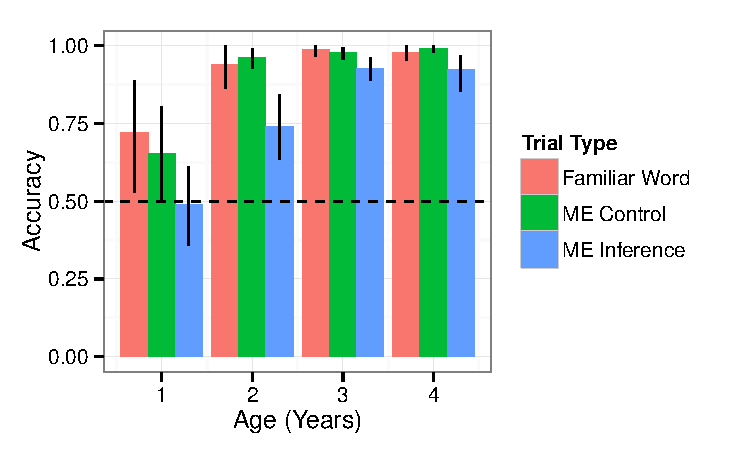
\includegraphics[width=5in]{figures/accuracy.pdf} 
    \caption{\label{fig:accuracy} Accuracy in our word recognition task, plotted by age group and trial type. Dashed line shows chance performance. Error bars show 95\% confidence intervals, computed by non-parametric bootstrap. }
  \end{center} 
\end{figure}

\subsubsection{Reaction times}

\begin{figure}[t] 
  \begin{center} 
    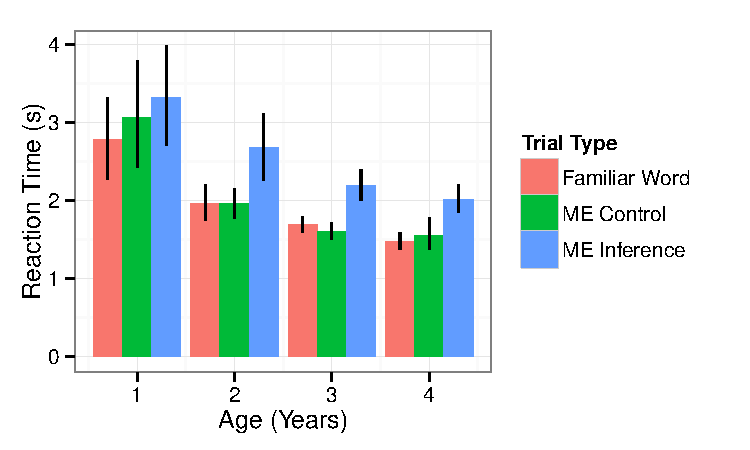
\includegraphics[width=5in]{figures/rt.pdf} 
    \caption{\label{fig:rt} Reaction times in our word recognition task, plotted by age group and trial type. Error bars show 95\% confidence intervals, computed by non-parametric bootstrap.}
  \end{center} 
\end{figure}


\begin{figure}[t] 
  \begin{center} 
    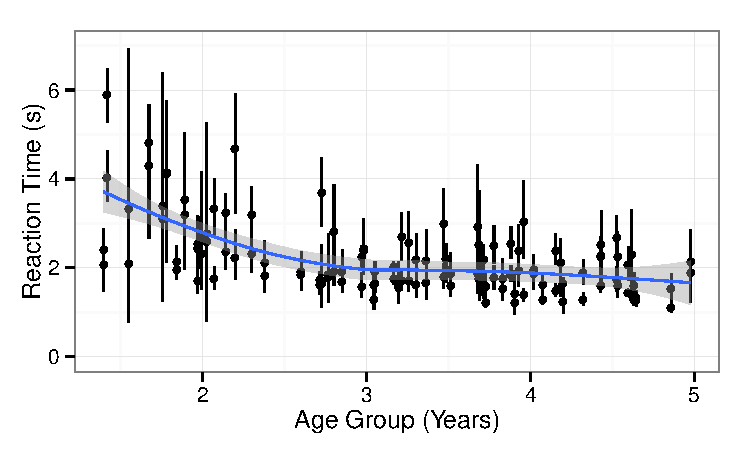
\includegraphics[width=5in]{figures/individuals.pdf} 
    \caption{\label{fig:rt} Reaction times for familiar word recognition (both Familiar and ME control trials), plotted by age. Each dot represents an individual. Error bars show 95\% confidence intervals on individual RTs, computed by non-parametric bootstrap. The smoothing line is a loess non-parametric regression line with a 95\% confidence interval.}
  \end{center} 
\end{figure}


\subsubsection{Reliabilities}

\section{Conclusions} 


\bibliographystyle{apacite}
\bibliography{tablet}

\end{document}
